\section{把 learning 图册读成同一台机器}

\begin{keyidea}
图里的方框不是都代表一颗芯片，线也不是都代表 PCB 上的一根铜线。整机学习图
把“物理部件、处理器接口、软件状态和宿主测试边界”放在同一张因果地图中；
读图的第一步不是沿箭头背名称，而是先确认每个对象属于哪一层、每条线表达哪种
事务。
\end{keyidea}

本书把 \filepath{docs/learning/} 中的七张整机学习图全部纳入对应章节。它们与
第二章的实体载板图承担不同职责：整机图解释 STUOS 在 QEMU PC 模型中看见的
逻辑硬件和软件交接，实体图解释 LattePanda Mu 载板上的真实器件引脚、电源和
PCB 网络。前者不能拿去布板，后者也不会自动证明内核已经实现设备驱动。

\subsection{一、先认清图中的四类对象}

\begin{longtable}{L{0.18\linewidth}L{0.27\linewidth}L{0.27\linewidth}L{0.18\linewidth}}
\toprule
对象 & 它在图中表示什么 & 它不表示什么 & 核对问题 \\
\midrule
硬件卡片 & CPU、ROM、RAM、PIC、PIT、UART、磁盘等可见设备 & C++ 类本身就是芯片 & 谁提供寄存器或存储行为 \\
软件卡片 & 固件、Stage 1、内核、驱动、进程与 Shell 的状态阶段 & PCB 上存在同名器件 & 代码在哪个特权级执行 \\
边界/泳道 & Host、Guest hardware、Ring 0、Ring 3 等所有权区域 & 只是为了美观的背景色 & 数据跨边界时由什么协议验证 \\
连接线 & 一类控制流、地址事务、端口事务、IRQ 或测试注入 & 默认都是一根可焊接导线 & 源、目的、方向和完成条件是什么 \\
\bottomrule
\end{longtable}

\term{泳道}{swimlane}是把同一层或同一责任主体放进一个横向区域的画法。例如
键盘图把 HOST、HARDWARE、KERNEL/RING 0、USER/RING 3 分开，强调一次按键
每跨过一条边界都要改变表示：宿主命令变成虚拟键盘事件，键盘事件变成扫描码，
扫描码经 IRQ 进入驱动，字符再经系统调用交给 Shell。

\term{卡片}{card}表示一个需要单独说明状态和接口的节点。它可能是一颗逻辑
设备，也可能是一段软件；判断标准要看卡片所在泳道和文字，不能只看矩形外观。

\subsection{二、四种线为什么绝不能混为一谈}

\begin{longtable}{L{0.16\linewidth}L{0.24\linewidth}L{0.31\linewidth}L{0.19\linewidth}}
\toprule
图中线型 & 表达的事务 & 典型例子 & 不能推出 \\
\midrule
绿色实线 & 内存/物理地址或 MMIO 访问 & CPU 取 ROM、访问 RAM、读 Local APIC & 图上是一条共享物理线 \\
蓝色虚线 & x86 独立 Port I/O 事务 & \code{IN/OUT} 到 COM1、PIT、PIC、ATA & 端口号等于物理内存地址 \\
红色实线 & 异步 IRQ 通知路径 & PIT/键盘到 PIC，再桥接到 Local APIC & 数据字节本身沿 IRQ 线传输 \\
紫色虚线 & 宿主控制、注入或验证 & QMP 注入按键、新 QEMU 进程重启验证 & 宿主绕过客户机设备和驱动 \\
\bottomrule
\end{longtable}

同一设备通常同时参加多类事务。i8042 的数据寄存器由蓝色 Port I/O 访问，
有字符就绪时又用红色 IRQ1 通知 CPU；扫描码存在控制器缓冲区，并不装在
IRQ 线上。把两条路径合并成“键盘连到 CPU”，就会无法解释为什么中断到了却
读不到数据，或者数据已在缓冲区却因为屏蔽 IRQ 而没有处理。

\begin{sidewaysfigure}[p]
  \centering
  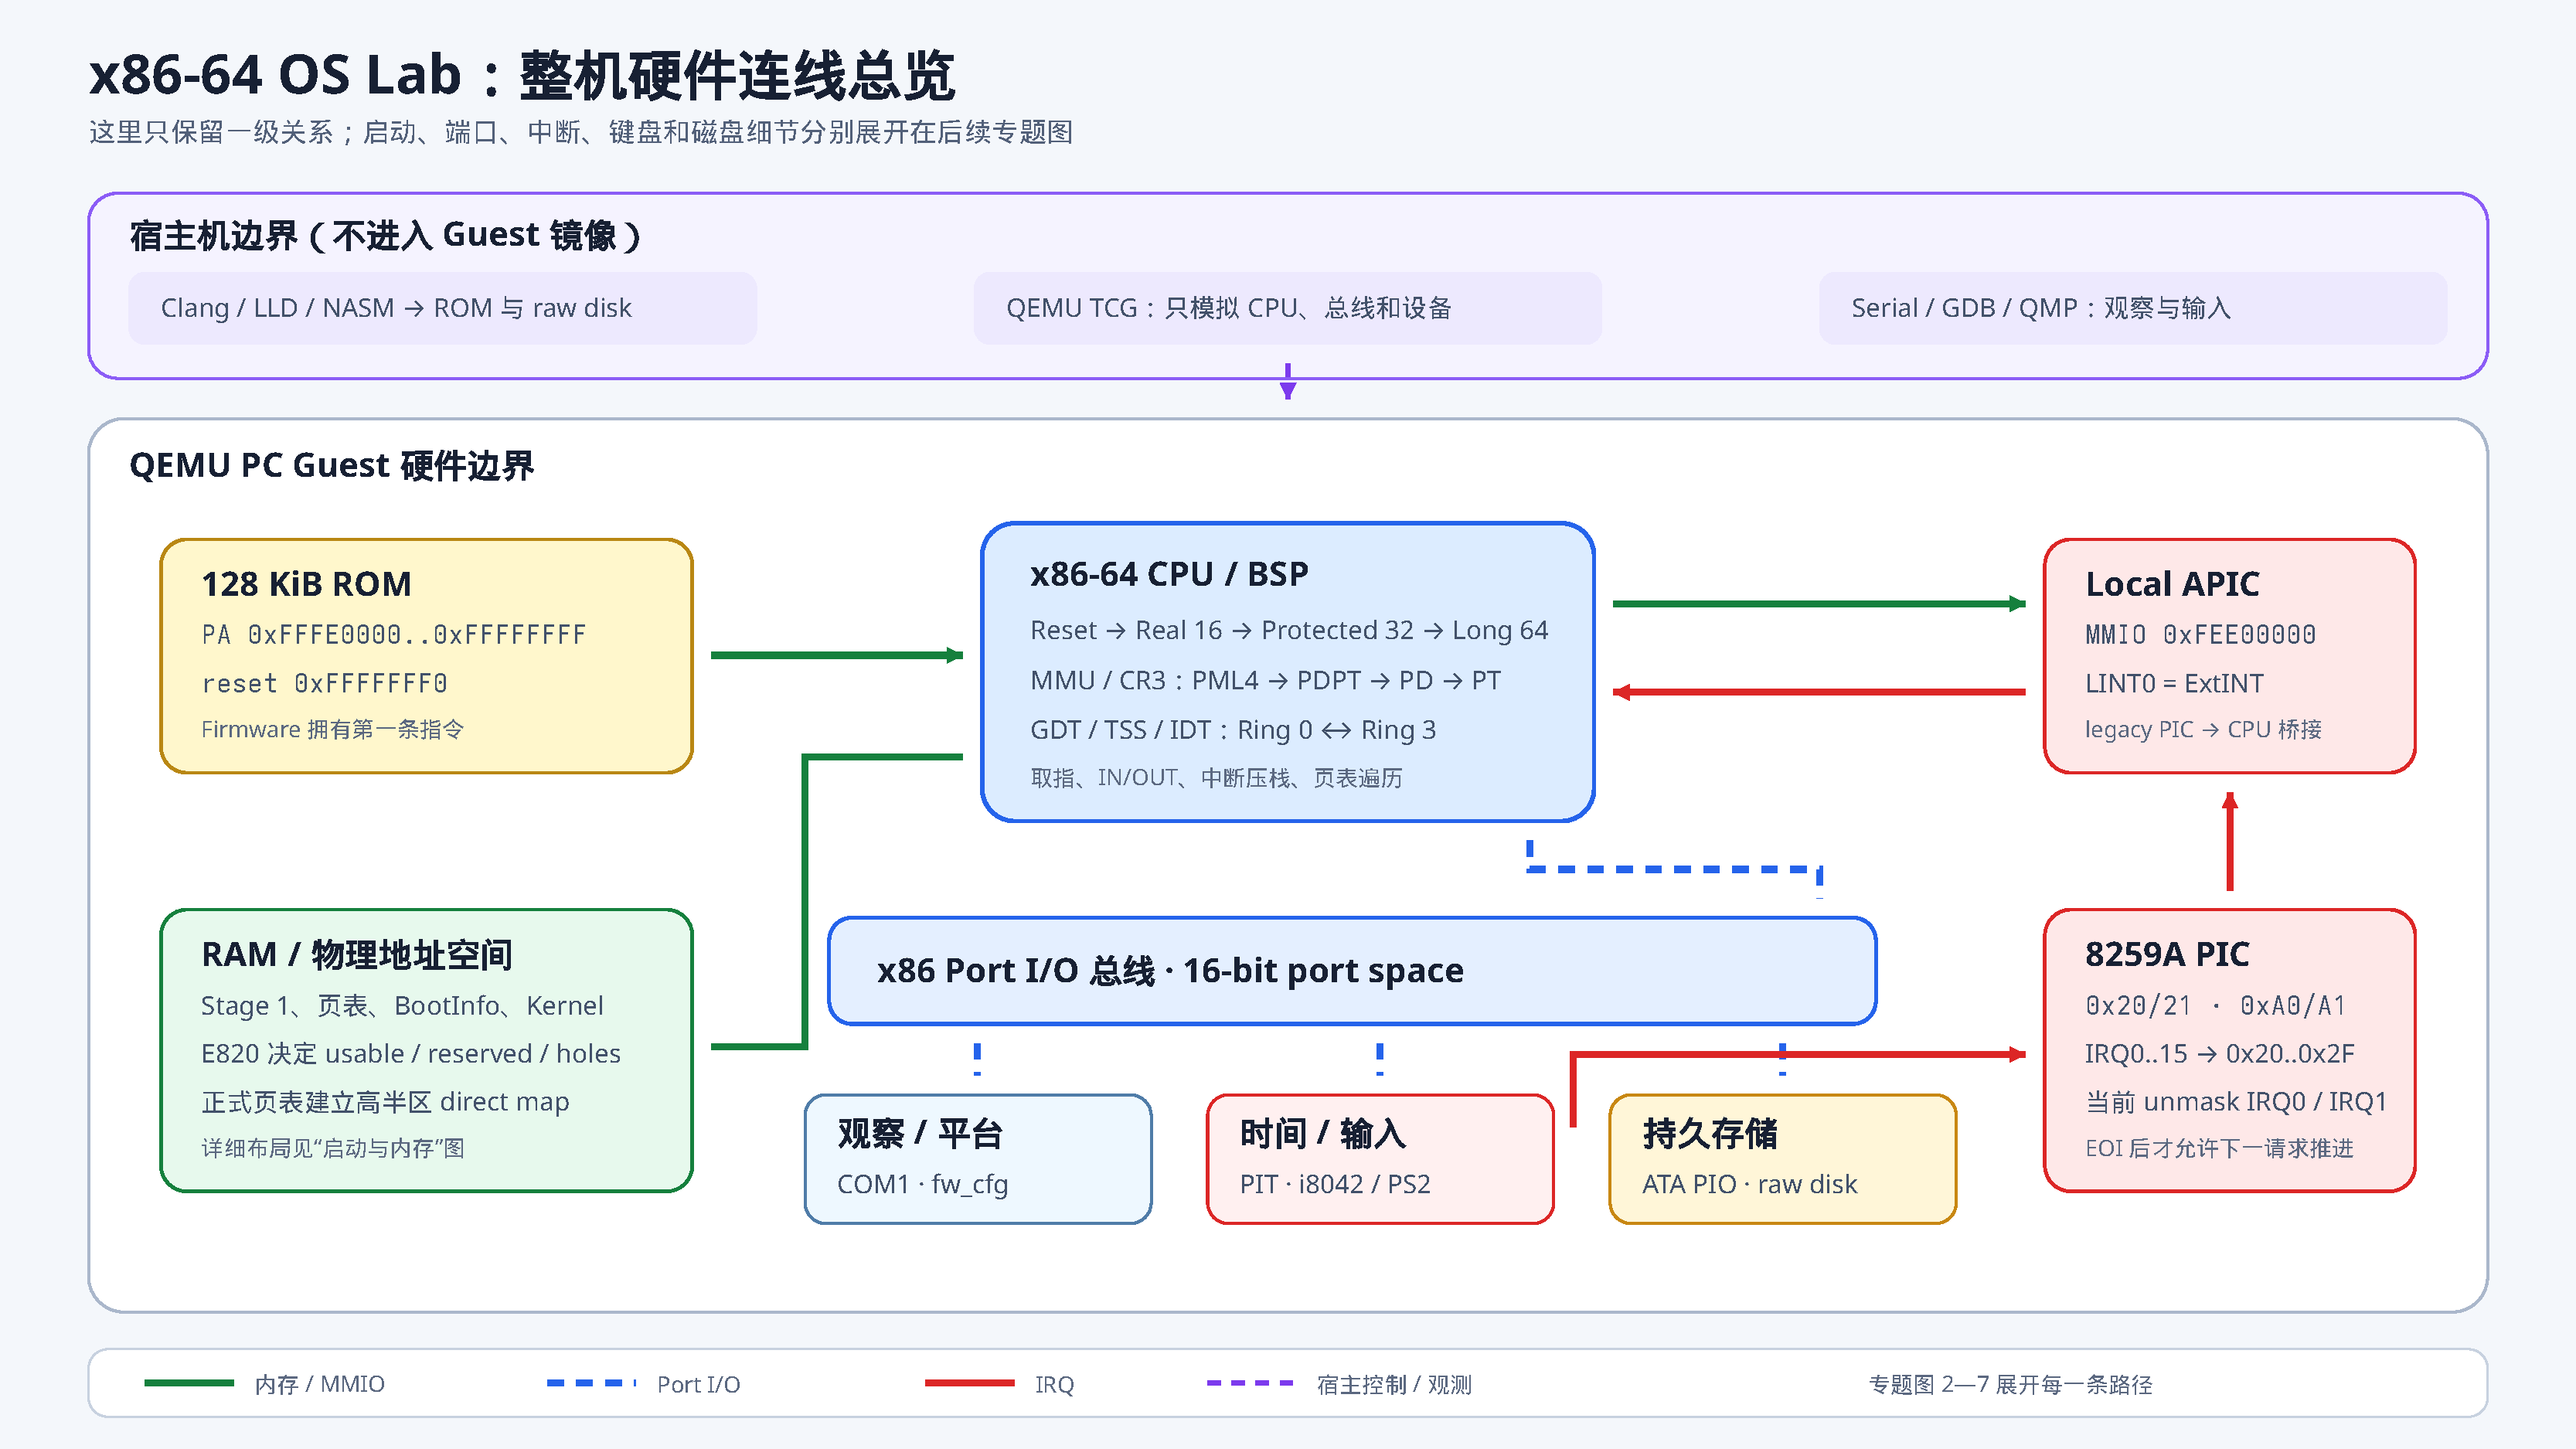
\includegraphics[width=0.96\textheight,height=0.82\textwidth,keepaspectratio]
    {figures/system_wiring/x86_64_os_hardware_wiring.pdf}
  \caption{STUOS 整机硬件连线总览。图中文字、线条和箭头均为矢量对象；
  横置整页用于保留可读字号。绿色、蓝色、红色和紫色分别表达不同事务，
  不能把它们当作一束同类导线。}
  \label{fig:system-wiring-overview}
\end{sidewaysfigure}
\clearpage

\subsection{三、沿整机总览逐块理解硬件}

\subsubsection{3.1 Host 为什么画在 Guest 外面}

\term{Host}{宿主}是运行构建工具和 QEMU 的现有系统；
\term{Guest}{客户机}是 QEMU 模拟出来、供 STUOS 使用的目标机器。Clang、
LLD、NASM 和镜像工具在宿主执行，产出 ROM 与 raw disk；它们不会随产物进入
客户机。Serial、GDB 和 QMP 也是宿主观察/控制接口，但它们观察的是客户机
状态或向设备模型提交事件。

QEMU TCG 位于宿主软件中，却对客户机实现 CPU、地址空间和设备规则。这里有
两个同时正确的描述：

\begin{itemize}[leftmargin=2em]
  \item 从宿主实现看，QEMU 是一个普通进程，设备模型是 C/C++ 代码；
  \item 从 STUOS 看，QEMU 提供的 ROM、RAM、PIC 和 ATA 就是它实际面对的硬件
        契约，目标代码不能直接调用宿主库跳过寄存器协议。
\end{itemize}

\subsubsection{3.2 ROM、RAM 和磁盘为什么画成三个部件}

ROM 保存断电后仍存在的最早固件字节，并被平台映射到复位可取指地址；RAM
保存运行时栈、页表、BootInfo 和已装入代码；磁盘保存按 LBA 编号的持久扇区。
CPU 可以直接从已映射 ROM/RAM 取指，却不能把 ATA 扇区号当作 RIP。完整搬运
路径是：
\[
\text{disk sector}
\rightarrow \text{ATA data register}
\rightarrow \text{CPU register}
\rightarrow \text{RAM}
\rightarrow \text{instruction fetch}.
\]

总览中的绿色线把 ROM、RAM、CPU 和 Local APIC 放在物理地址/MMIO 一侧，
并不意味着三者电气相同。ROM 拒绝普通写入，RAM 可读写，Local APIC 寄存器
具有副作用；平台地址译码只是在同一个地址事务入口上把范围分给不同响应者。

\subsubsection{3.3 CPU 方框为什么同时出现 MMU、描述符表和 Ring}

CPU 不只做算术。MMU 根据 CR3 和页表翻译地址；GDT/TSS/IDT 给特权转换和事件
入口提供处理器可验证的数据结构；RIP/RSP/RFLAGS 与控制寄存器共同决定下一条
指令在哪里、使用哪个栈、是否接受可屏蔽中断。这些结构多数存放在 RAM 中，
CPU 寄存器只保存入口、根地址或当前选择状态。

\subsubsection{3.4 Port I/O 总线是架构空间，不是一根现代排线}

图中央的 Port I/O 粗线把 COM1、PIT、i8042、ATA 和 PIC 汇在一起，表示它们
都由 \code{IN}/\code{OUT} 指令和 16 位端口号访问。真实芯片内部可由不同片上
互连或兼容逻辑实现；QEMU 则由各设备模型响应相应端口。粗线是软件可见接口的
集合，不宣称主板上存在一根标着“Port I/O”的铜排。

\subsubsection{3.5 PIC 与 Local APIC 为什么同时存在}

8259A PIC 接收传统 IRQ0/IRQ1，经过初始化后把它们映射为向量
\code{0x20}/\code{0x21}。本项目使用 virtual-wire 路径把 PIC 的 INTR
经 Local APIC LINT0/ExtINT 交给 BSP。蓝色端口线用于配置 PIC，红色 IRQ
线用于报告事件，绿色 MMIO 线用于配置 Local APIC；三条线共同存在才构成
完整中断路径。

\subsection{四、路线图不是版本纪念册，而是依赖图}

\begin{sidewaysfigure}[p]
  \centering
  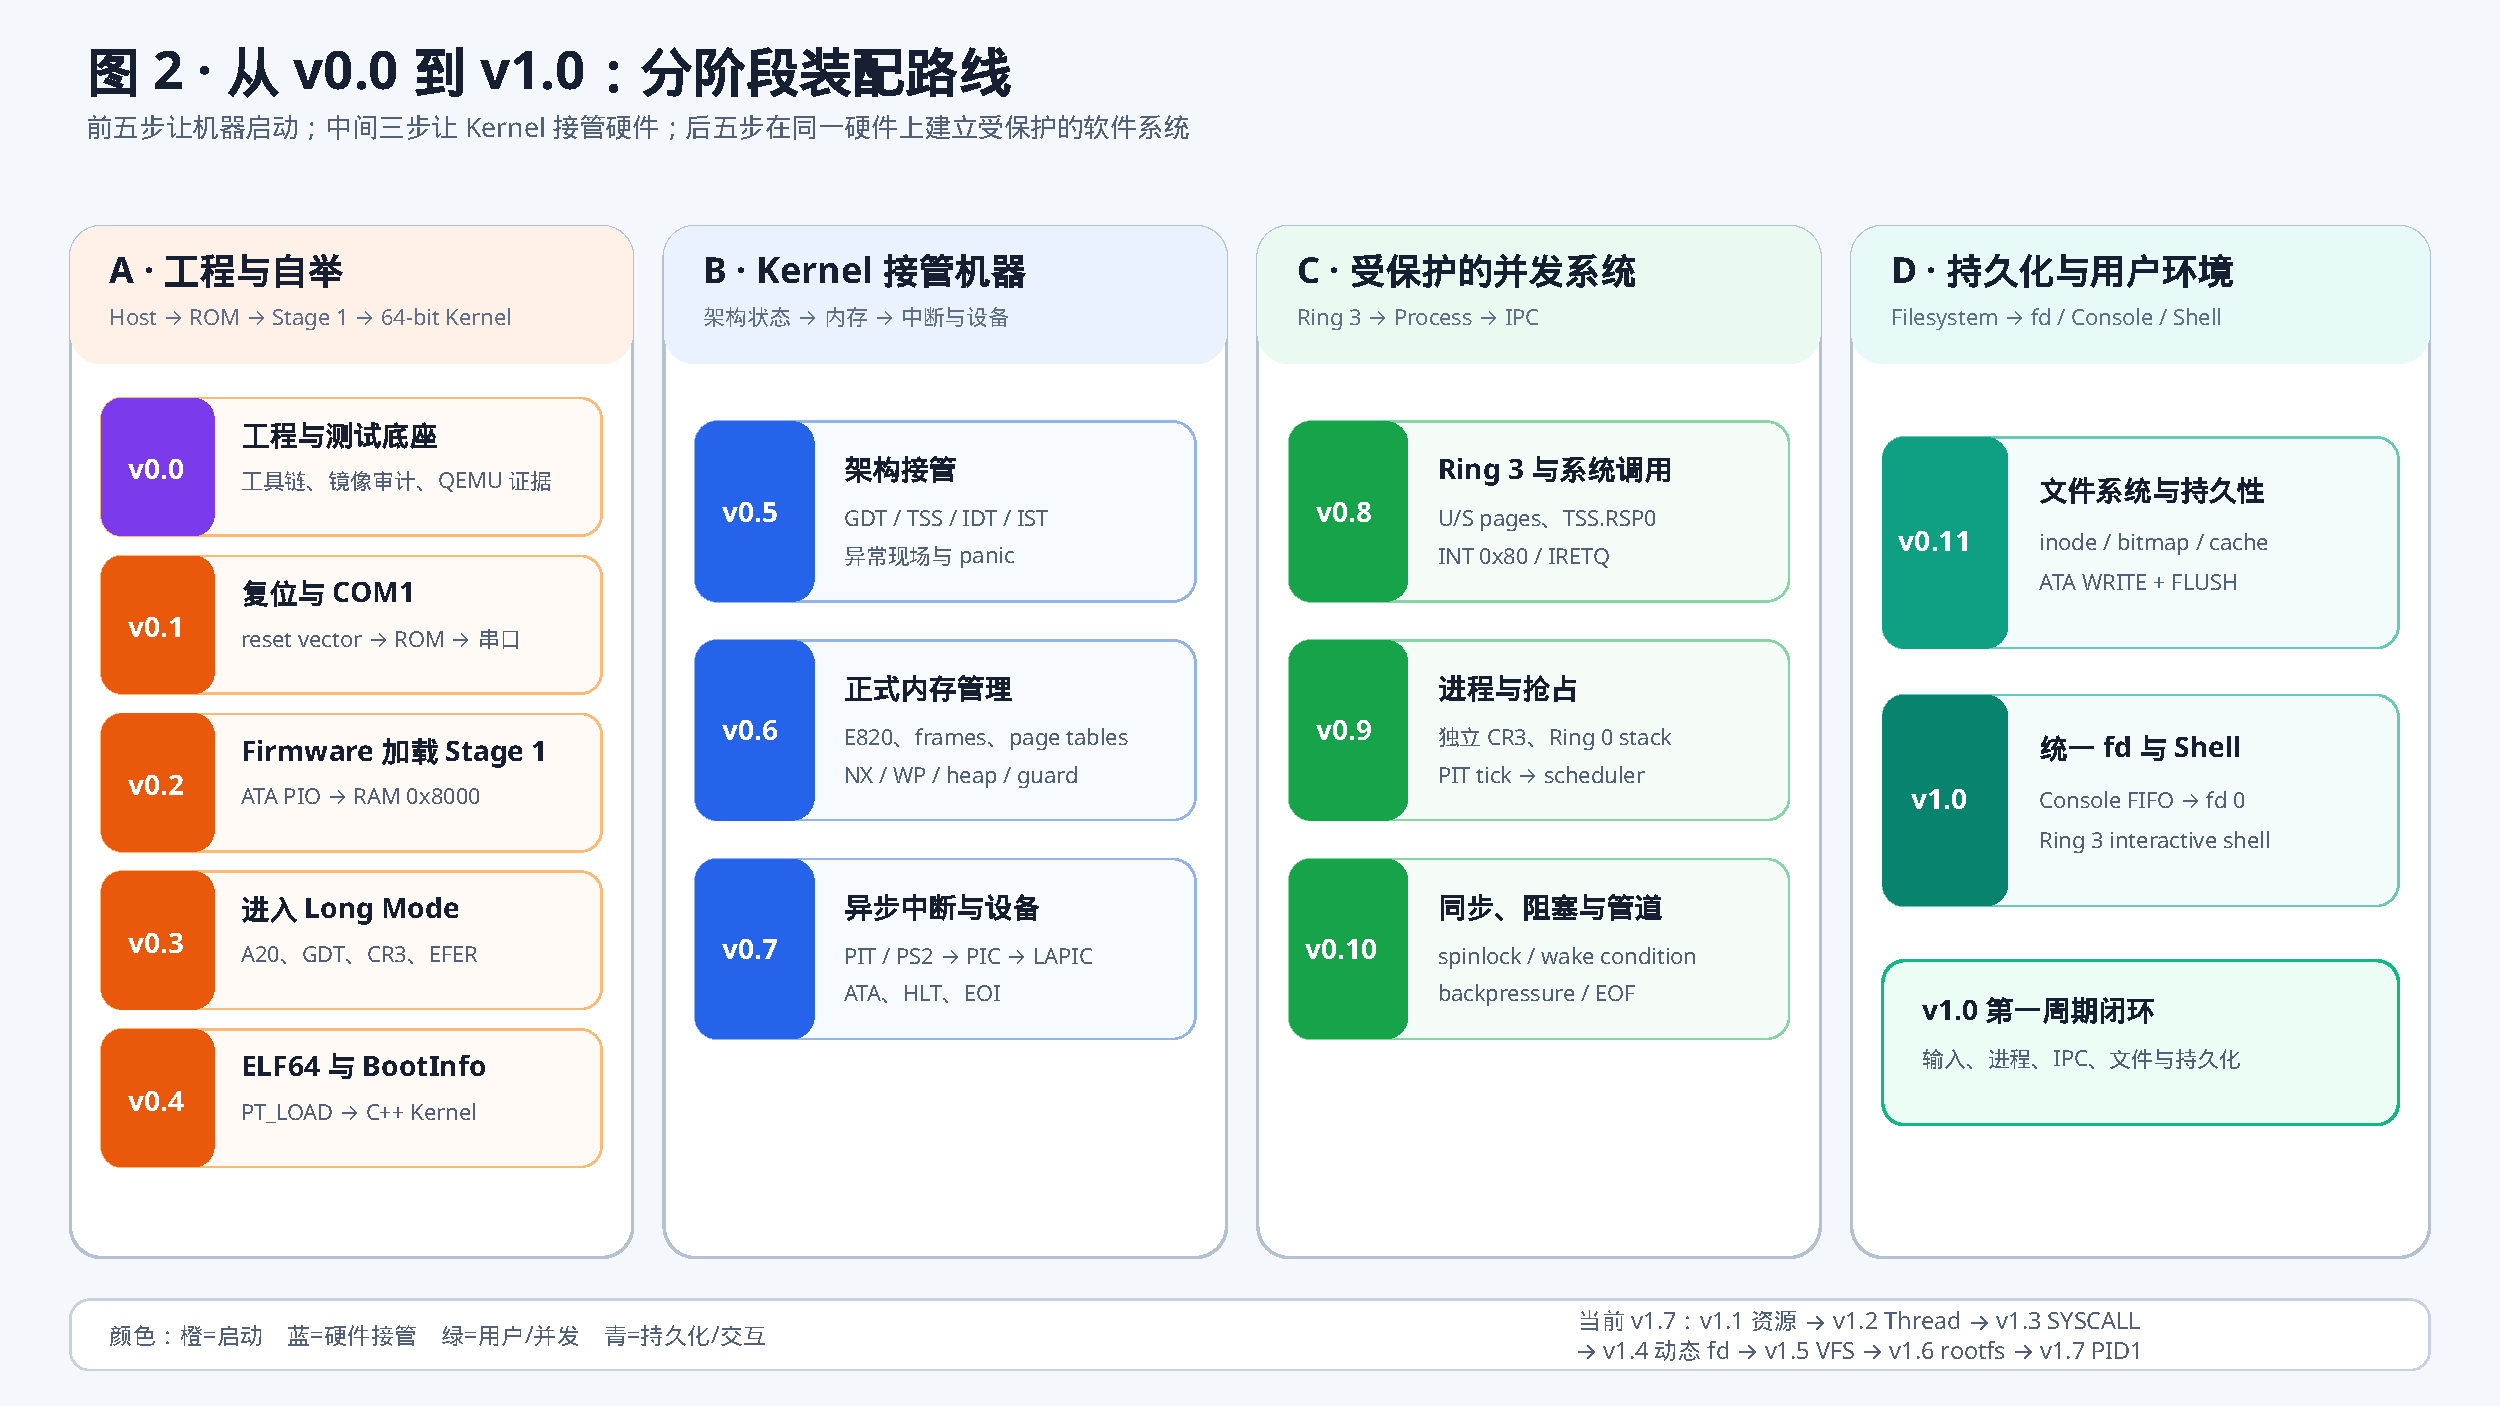
\includegraphics[width=0.96\textheight,height=0.82\textwidth,keepaspectratio]
    {figures/system_wiring/hardware_stage_roadmap.pdf}
  \caption{从 v0.0 到 v1.0 的十三个可验收增量。每张卡片表示新建立的一组
  前置条件；箭头方向是能力依赖，不表示后续版本删除旧机制。图下方同时标明
  当前 v1.1--v1.6 的资源、Thread、SYSCALL、动态文件表、VFS 与 rootfs v2 增量。}
  \label{fig:hardware-stage-roadmap}
\end{sidewaysfigure}
\clearpage

路线图把第一周期分成四组，不是为了按颜色记忆，而是为了防止同时打开太多
不可观测状态：

\begin{longtable}{L{0.14\linewidth}L{0.21\linewidth}L{0.30\linewidth}L{0.25\linewidth}}
\toprule
阶段 & 增量 & 新获得的能力 & 为什么不能提前 \\
\midrule
A 工程与自举 & v0.0--v0.4 & 可复现构建、ROM、串口、Stage 1、长模式、ELF 与 BootInfo & 没有前一层便无法观察或装入后一层 \\
B Kernel 接管 & v0.5--v0.7 & GDT/TSS/IDT、物理内存、页表、异常、中断和设备 & 内核先要能隔离故障，才适合接受异步事件 \\
C 受保护并发 & v0.8--v0.10 & Ring 3、系统调用、进程、抢占、阻塞与 IPC & 用户边界依赖页权限、内核栈和异常入口 \\
D 持久化与交互 & v0.11--v1.0 & 文件系统、统一 fd、控制台与 Shell & 交互命令要依赖调度、驱动和持久对象的完整链 \\
\bottomrule
\end{longtable}

\topic{“后续能力”不会让早期硬件消失}%
v1.0 的 Shell 打印一个字符，仍要依赖 v0.1 建立的 UART；读取文件仍要依赖
v0.2 开始使用的 ATA；进入 Ring 3 仍要依赖 v0.3 的模式转换和 v0.5 的
描述符表。版本号表达的是第一次建立某项能力，不是该能力只在那个版本存在。

\topic{v1.1--v1.6 为什么画在第一周期之后}%
v1.1 收口可回收内核资源，v1.2 把 Process 与 Thread 分离，v1.3 加入原生
SYSCALL/SYSRET 与 CPU-local，v1.4 建立类型化 KernelObject、共享
FileDescription 和动态 FileTable，v1.5 再建立 VFS、挂载与 memfs，v1.6
则让 rootfs v2 承担可扩展持久化与完整命名空间修改。它们在
v1.0 已闭合的启动、用户、文件和
测试链上继续强化生命周期与接口，不改写“先有机器状态，后有软件抽象”的依赖
方向。

\subsection{五、读任意一张硬件学习图的七问法}

后续看到更复杂的图，可以逐节点回答七个问题：

\begin{enumerate}[leftmargin=2.2em]
  \item 这个框是物理器件、架构状态、软件对象，还是宿主工具？
  \item 输入从哪里来，输出到哪里去，方向是否会反转？
  \item 线表示数据搬运、控制流、地址事务、中断请求，还是测试控制？
  \item 这一步由固件、引导器、内核、驱动还是用户程序初始化？
  \item 完成条件由哪个状态位、寄存器、返回值或测试标记证明？
  \item 失败时数据还归谁，是否需要回滚、清中断、释放内存或保持磁盘不变？
  \item 把 QEMU 换成实体平台后，哪个接口保持，哪个地址、设备或固件假设必须
        重新发现？
\end{enumerate}

如果七问中有一项只能回答“反正箭头连着”，说明图还没有读成工程契约。后续
六张整机专题图会分别把启动/内存、Port I/O、中断、键盘和持久化路径放大，
第二章实体案例再把电源、差分对和引脚真正落到 PCB 网络。
